

\documentclass[paper=a4, fontsize=11pt]{article} % A4 paper and 11pt font size

\usepackage[T1]{fontenc} % Use 8-bit encoding that has 256 glyphs
\usepackage[english]{babel} % English language/hyphenation
\usepackage{amsmath,amsfonts,amsthm} % Math packages
\usepackage{xcolor}
\usepackage{caption}
\usepackage{bashful}
\usepackage{empheq}
\usepackage{graphicx}
\usepackage{cancel}
\usepackage[shortlabels]{enumitem}
\usepackage[symbol]{footmisc}
\renewcommand{\thefootnote}{\fnsymbol{footnote}}
\newcommand*{\vertbar}{\rule[-1ex]{0.5pt}{2.5ex}}
\usepackage{titlesec}

\titleformat{\section}
  {\normalfont\Large\bfseries}{\thesection.}{1em}{}

%----------------------------------------------------------------------------------------
%	TITLE SECTION
%----------------------------------------------------------------------------------------

\newcommand{\horrule}[1]{\rule{\linewidth}{#1}} % Create horizontal rule command with 1 argument of height

\title{
\horrule{1pt} \\[0.4cm] % Thick top horizontal rule
 \Large Linear analysis of sub-shelf channel and keel formation
\horrule{1pt} \\[0.5cm] % Thick bottom horizontal rule
}

\author{Aaron Stubblefield} % Your name

\date{\small\today} % Today's date or a custom date

\begin{document}

\maketitle % Print the title

\setcounter{footnote}{1}

\section{Model}
Here, we analyze a small-perturbation model for ice shelves undergoing localized basal melting and/or freezing.
The model is derived in the appendix.
The variables in the small-perturbation model are
\begin{align*}
&h = \text{upper-surface elevation perturbation}\\
&s = \text{lower-surface elevation perturbation}\\
&m = \text{melting (or freezing) rate perturbation}.
\end{align*}
These perturbations are relative to a background state corresponding to uniform
flow in the $x$ direction and perfect flotation (Figure \ref{fig:sketch}). We will also be interested in velocity perturbations (`secondary flow')
$\pmb{u}=[u,v,w]^T$ relative to this background state.

Throughout these notes, we will refer to the condition $$h=-\delta s$$ as the ``perfect
flotation condition'' where $$\delta = \rho_\mathrm{w}/\rho_\mathrm{i}-1$$
is the flotation factor. One of our goals is to analyze how well the solutions satisfy this condition.
We will also be interested in the depth-dependence of the horizontal velocity perturbations $u$ and $v$---
the assumption that the depth-averaged ice velocity (i.e. ice flux) matches
its surface value underlies traditional melt-rate estimation methods.


\begin{figure}
  \centering
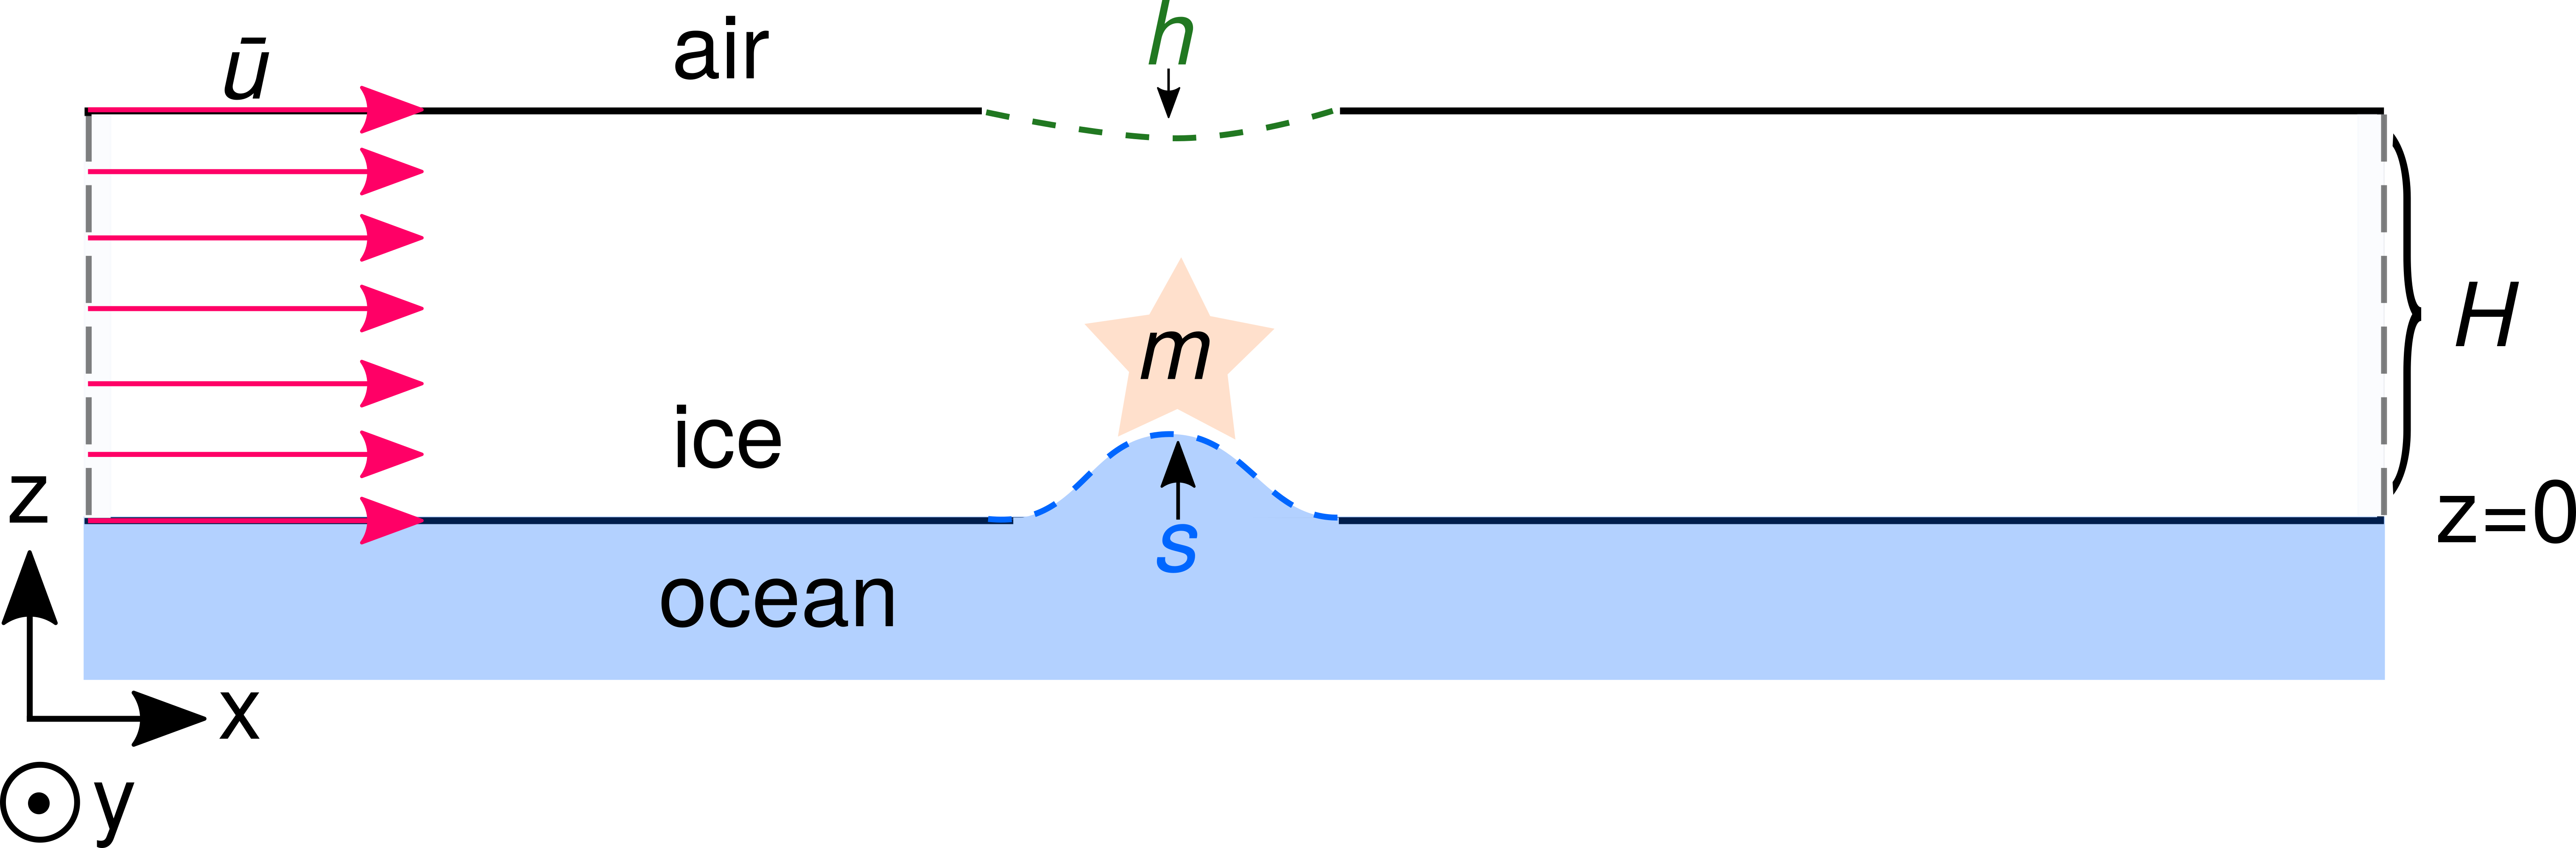
\includegraphics[width=0.95\textwidth]{figs/fig1.png}
\caption{Sketch of model variables.}
\label{fig:sketch}
\end{figure}

We use the Fourier transform (denoted with $\;\widehat{}\;$) with respect to the horizontal coordinates $(x,y)$
to solve the problem. To this end, we define
\begin{align*}
[k_x,k_y]^T = \text{wavevector},\quad
k = \sqrt{k_x^2 + k_y^2},\quad
k' = Hk,
\end{align*}
where $H$ is the ice thickness.
The Fourier-transformed elevations evolve according to
the coupled system
\begin{eqnarray}
&&\frac{\partial \widehat{h}}{\partial t}+ \left[ik_x \bar{u}  + \mathsf{R}\right]\widehat{h} = -\mathsf{B}\delta\widehat{s}\label{hf}\\
&&\frac{\partial \widehat{s}}{\partial t}+ [ik_x \bar{u} + \delta\mathsf{R}]\widehat{s} = \widehat{m} - \mathsf{B} \widehat{h}, \label{sf}
\end{eqnarray}
where $\bar{u}$ is the background ice flow speed (Appendix). The function
\begin{eqnarray}
\mathsf{R} = \left(\frac{\rho_\mathrm{i} g}{2\eta k}\right) \frac{e^{4{k'}} +4{k'} e^{2{k'}} -1 }{e^{4{k'}} -2(1+2{k'}^2)e^{2{k'}} +1}, \label{Rf}
\end{eqnarray}
describes viscous relaxation of surface topography and influences both the upper and basal surfaces.

Buoyancy forcing between the upper and basal surfaces is described by the function
\begin{eqnarray}
\mathsf{B} = \left(\frac{\rho_\mathrm{i} g}{2\eta k}\right) \frac{ 2({k'}+1)e^{3{k'}}+2({k'}-1)e^{{k'}} }{e^{4{k'}} -2(1+2{k'}^2)e^{2{k'}} +1}. \label{B}
\end{eqnarray}
The upper-surface evolution equation (\ref{hf}) shows that a change in $s$ forces changes in $h$ proportional to the
buoyancy function $\mathsf{B} $ (eq. \ref{B}), and vice versa for the basal-surface evolution equation (\ref{sf}).
On the other hand, $\mathsf{R}$ causes these surface perturbations to decay. The balance between
these relaxation and buoyancy functions is intimately linked to the stability of sub-shelf channels and keels.
Figure (\ref{fig:RB}) shows plots of the buoyancy and relaxation functions, and some of their
limiting properties.

The relaxation and buoyancy functions are singular in the limit
$k\to 0$ (Figure 2). This means that
relaxation and buoyancy adjustments occur \emph{instantaneously} at long wavelengths under the assumption of
an infinitely expansive ice shelf. In reality, the ice shelf is partially supported by the grounded
portion of the ice sheet (well, until it breaks off...), which ameliorates this behavior.
After scaling the problem, we introduce regularizations to avoid these singularities when computing the solutions.

\section{Scaling}
Now, we introduce scalings for the model equations (\ref{hf}) and (\ref{sf}).
We scale the variables according to
\begin{eqnarray}
  && x = Hx',\quad y=Hy',\quad z=Hz', \quad t = t_r t', \nonumber \\
&&k = H^{-1}k' , \quad k_x = H^{-1}k_x', \quad k_y  = H^{-1}k_y', \nonumber\\
&&u = \frac{H}{t_r}u',\quad v = \frac{H}{t_r}v',\quad w = \frac{H}{t_r}w',\nonumber\\
&& h = H h', \quad s = H s' ,\quad m = \frac{H}{t_r} m' \label{scaling}
\end{eqnarray}
where primes denote dimensionless quantites and
\begin{eqnarray}
t_r \equiv \frac{2\eta}{\rho_i gH} \label{t_relax}
\end{eqnarray}
is the characteristic timescale for viscous relaxation of surface topography.

We scale the relaxation frequency function (eq. \ref{Rf}) according to
\begin{eqnarray}
   &&\mathsf{R} = t_r^{-1} \mathsf{R}', \quad
 \mathsf{R}'(k') =  \frac{1}{k'}\frac{e^{4k'} +4k' e^{2k'} -1 }{e^{4k'} -2(1+2(k')^2)e^{2k'} +1}. \label{Rfsc}
\end{eqnarray}
Similarly, we scale the buoyancy transfer function according to
\begin{eqnarray}
   &&\mathsf{B} =  t_r^{-1} \mathsf{B}', \quad
 \mathsf{B}'(k') =   \frac{1}{k'}\frac{ 2(k'+1)e^{3k'}+2(k'-1)e^{k'} }{e^{4k'} -2(1+2(k')^2)e^{2k'} +1}. \label{Bsc}
\end{eqnarray}
Omitting primes on the variables, the evolution equations (\ref{hf}) and (\ref{sf}) scale to
\begin{eqnarray}
&&\frac{\partial \widehat{h}}{\partial t}+ \left[ik_x {\alpha}  +  \mathsf{R}\right]\widehat{h} = - \mathsf{B}\delta\widehat{s}\label{hfsc}\\
&&\frac{\partial \widehat{s}}{\partial t}+ [ik_x{\alpha}  + \delta \mathsf{R}]\widehat{s} = \widehat{m} -  \mathsf{B} \widehat{h},\label{sfsc}
\end{eqnarray}
where
\begin{equation}
\alpha = \frac{\bar{u} t_r}{H}  \label{uh_eq}
\end{equation}
is the background flow speed relative the the characteristic velocity scale
$H/t_r$.

\begin{figure}
  \centering
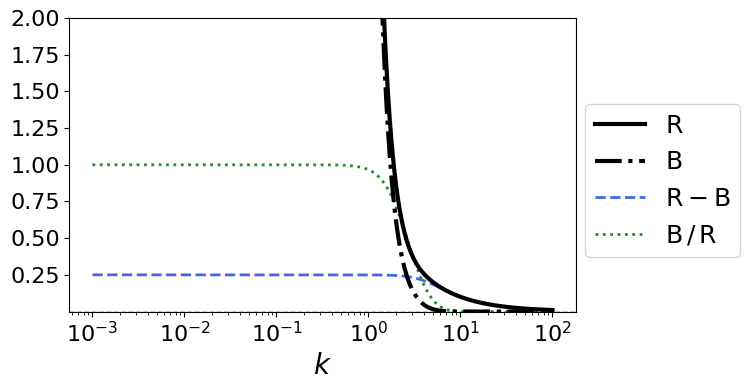
\includegraphics[width=0.95\textwidth]{figs/fig2.png}
\caption{Graphs of (scaled) $\mathsf{R}$ (eq. \ref{Rfsc}) and $\mathsf{B}$ (eq. \ref{Bsc}), as well as their difference and quotient. The limits $\mathsf{R}-\mathsf{B}\to 1/4$ and $\mathsf{R}/\mathsf{B}\to 1$
as $k\to 0$ can be proven using L'Hospital's rule.}
\label{fig:RB}
\end{figure}

\section{Regularization}
To remove the singularities in $\mathsf{R}$ and $\mathsf{B}$, we define the regularized
relaxation and buoyancy functions
\begin{eqnarray}
\mathsf{R}_\varepsilon = (\varepsilon + \mathsf{R}^{-1})^{-1}\\
\mathsf{B}_\varepsilon = (\varepsilon + \mathsf{B}^{-1})^{-1},
\end{eqnarray}
where $\varepsilon$ is a small regularization parameter. We choose
$\varepsilon$ such that the $k\to 0$ limit $\mathsf{R}_\varepsilon-\mathsf{B}_\varepsilon\to
\frac{1}{4}$ (Figure \ref{fig:RB}) is attained at $k = 10^{-3}$, resulting in
$\varepsilon \approx 2.5\times 10^{-14}$. This results in other analytical
limits in the problem being respected at small $k$ (see
below), so we think that this is a good idea and we don't feel bad about it.
These regularizations are only used to facilitate computation of the solutions
so there are no $\varepsilon$'s appearing in the analysis below.


\section{Analysis}

\subsection{Solution formulas}
We rewrite the system (\ref{hfsc})-(\ref{sfsc}) as
\begin{eqnarray}
\frac{\partial\pmb{y}}{\partial t} = \mathsf{A}\pmb{y} + \pmb{b}, \label{ydot}
\end{eqnarray}
where
\begin{eqnarray}
\pmb{y} = \left[\begin{array}{ll}
\widehat{h} \\
\widehat{s}
\end{array}\right], \quad
\pmb{b} =
\left[\begin{array}{ll}
0\\
\widehat{m}
\end{array}\right],\quad
\mathsf{A} =-\left[\begin{array}{ll}
ik_x{\alpha}+ \mathsf{R} & \delta\mathsf{B} \\
\mathsf{B} & ik_x{\alpha}+\delta \mathsf{R}
\end{array}\right],
\label{Amat}
\end{eqnarray}
with the matrix $\mathsf{A}$ not depending on time $t$.
We diagonalize $\mathsf{A}$ according to
\begin{eqnarray}
&& \mathsf{A} = \mathsf{P}\mathsf{D}\mathsf{P}^{-1},\quad
 \mathsf{P} = \left[\begin{array}{cc}
\vertbar & \vertbar \\
\pmb{\varphi}_- & \pmb{\varphi}_+ \\
\vertbar & \vertbar
\end{array}\right],\quad
 \mathsf{D} = \left[\begin{array}{ll}
\lambda_-  & 0 \\
0 & \lambda_+
\end{array}\right].
\end{eqnarray}
The eigenvalues ($\lambda_\pm$) and eigenvectors ($\pmb{\varphi}_\pm$)
of $\mathsf{A}$ are
\begin{eqnarray}
&&\lambda_\pm = -ik_x{\alpha}-\frac{\delta+1}{2} \mathsf{R} \pm \frac{\mu}{2} \label{Lambda} \\
&&\pmb{\varphi}_\pm = \left[\begin{array}{c}
\frac{\mathsf{R}(1-\delta)\mp\mu}{2\mathsf{B}} \\
 1
\end{array}\right]
\end{eqnarray}
where we have defined
\begin{equation}
\mu = \sqrt{4\delta\mathsf{B}^2 +  \mathsf{R}^2(\delta-1)^2}.
\end{equation}

See Figure \ref{fig:eigvals} for graphs of the real parts of the eigenvalues and Figure \ref{fig:eigvecs}
for graphs of the (normalized) eigenvector components over a range of $k$.
The main points are that
\begin{itemize}
\item the real parts of the eigenvalues are always negative---meaning that the
steady solutions are stable. In particular, $\lambda_+$ remains bounded as $k\to 0$
so that $\pmb{\varphi}_+$ becomes the dominant mode in the long-wavelength limit.
\item the eigenvector corresponding to the dominant (larger)
eigenvalue $\lambda_+$ has the limit $\pmb{\varphi}_+/\|\pmb{\varphi}_+\|\to [-\delta,1]^T$,
which drives the solution towards the perfect flotation condition. The other
eigenpair encourages deviations from perfect flotation, but this effect
decays as $k\to 0$ since $\lambda_-$ becomes very negative. However, it is still
important at shorter wavelengths.
\item The normalized eigenvectors approach $\pmb{\varphi}_+/\|\pmb{\varphi}_+\| \to [0,1]^T$ and $\pmb{\varphi}_-/\|\pmb{\varphi}_-\|\to [1,0]^T$
as $k\to \infty$, meaning that the surface and basal response becomes decoupled
at short wavelengths.
This just means that short-wavelength perturbations are not transmitted through the ice.
\end{itemize}

\begin{figure}
  \centering
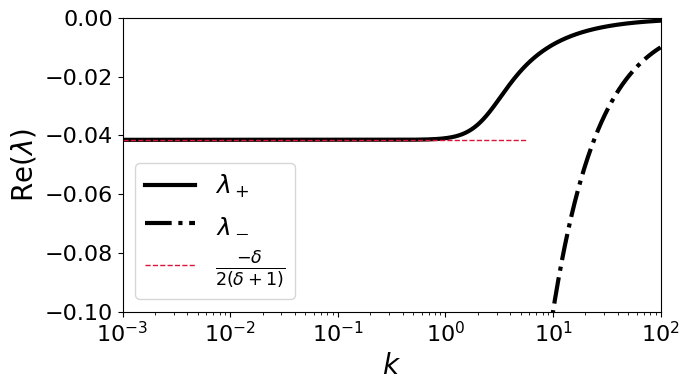
\includegraphics[width=0.95\textwidth]{figs/fig3.png}
\caption{Real parts of eigenvalues of $\mathsf{A}$.}
\label{fig:eigvals}
\end{figure}

\begin{figure}
\centering
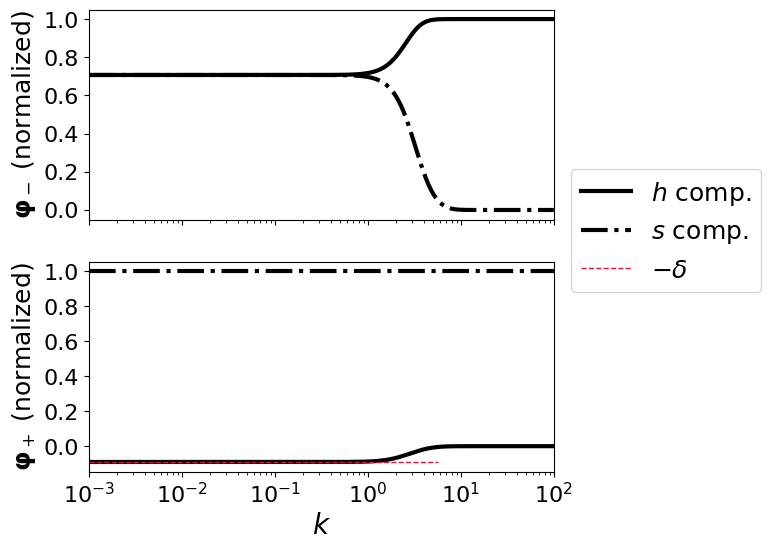
\includegraphics[width=0.95\textwidth]{figs/fig4.png}
\caption{Normalized eigenvectors $\pmb{\varphi}_\pm$ of $\mathsf{A}$. `$h$ comp.' is the first
vector component and `$s$ comp.' is the second component. Note that $\pmb{\varphi}_+\to[-\delta,1]^T$
as $k\to 0$, corresponding to the perfect flotation condition. }
\label{fig:eigvecs}
\end{figure}


\subsubsection{General solutions}
Assuming no initial perturbation ($\pmb{y}(0)=\pmb{0}$), the solution to (\ref{ydot}) is
\begin{eqnarray}
\pmb{y}(t) = \int_0^t e^{\mathsf{A}(t-\tau)} \pmb{b}(\tau)\;\mathrm{d}\tau, \label{ysol}
\end{eqnarray}
where $e^{\mathsf{A}t} = \mathsf{P}e^{\mathsf{D}t}\mathsf{P}^{-1}$ is the matrix exponential.
Using (\ref{ysol}), we find that
the solution for the ice-surface elevation anomaly is
\begin{eqnarray}
&&\widehat{h} = \widehat{m} * {\mathsf{K}}_h \nonumber, \\
&&{\mathsf{K}}_h  \equiv  -\frac{\delta\mathsf{B}}{\mu}(e^{\lambda_+ t}-e^{\lambda_-t}), \label{hfsol}
\end{eqnarray}
where $*$ denotes convolution over time. Similarly, the solution for the lower-surface elevation anomaly is
\begin{eqnarray}
  &&\widehat{s} = \widehat{m} * {\mathsf{K}}_s\nonumber, \\
 &&{\mathsf{K}}_s  \equiv  \frac{1}{2\mu}[(\mu-\chi)e^{\lambda_- t}+(\mu+\chi)e^{\lambda_+t}],\nonumber \\
  &&\chi \equiv (1-\delta)\mathsf{R}. \label{sfsol}
\end{eqnarray}
From these solution formulas we can see that $h$ will be close to $-\delta s$ provided that
$\mathsf{K}_h$ is close to $-\delta \mathsf{K}_s$ and $|m|$ is not too large\footnote{
More precisely, over some time frame $[0,T]$, we can use Young's convolution inequality,
H\"{o}lder's inequality, and the Plancherel theorem to estimate the deviation from
perfect flotation ($h=-\delta s$) via (skipping the details)
\begin{equation*}
\|h+\delta s\|_{2,2} \leq \|\mathsf{K}_h + \delta \mathsf{K}_s\|_{1,\infty} \times \|m\|_{2,2}
\end{equation*}
where we have defined the mixed Lebesgue norm of a function $f(x,y,t)$---or $f(k_x,k_y,t)$---by
\begin{equation*}
\|f\|_{p,q} = \left(\int_0^T \|f\|_{L^q(\mathbb{R}^2)}^p \; \mathrm{d}t \right)^{\frac{1}{p}}.
\end{equation*}
}.
We show the kernels $\mathsf{K}_s$ and $-\mathsf{K}_h/\delta$ in Figure \ref{fig:kernels},
highlighting that $\mathsf{K}_h(k,t)\approx-\delta\mathsf{K}_s(k,t)$ when
$(k,t)\in(0,1)\times(10^{-1},\infty)$. Therefore, and unsuprisingly,
significant deviations from perfect flotation only occur on fast timescales (relative to the relaxation time)
and short wavelengths (relative to ice thickness). We show an example of this short-wavelength
deviation in Figure \ref{fig:keel2}.


\begin{figure}
  \centering
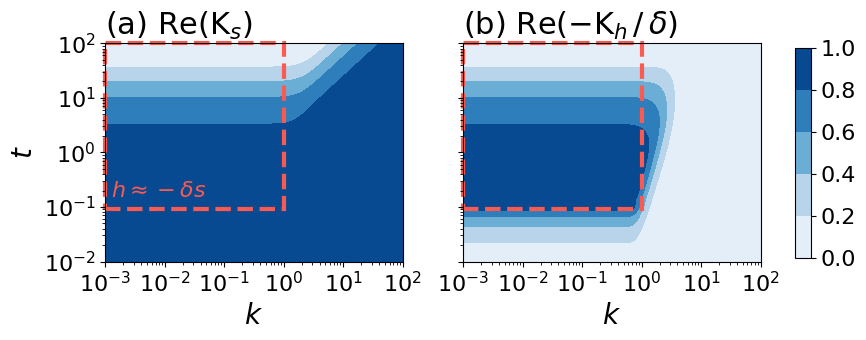
\includegraphics[width=0.99\textwidth]{figs/fig5.png}
\caption{Real parts of the kernels $\mathsf{K}_s$ and $-\mathsf{K}_h/\delta$ of the solution operator.
The dashed boxes denote the region in $(k,t)$ space where the flotation thickness is approximately satisfied
since $\mathsf{K}_h\approx -\delta \mathsf{K}_s$ .}
\label{fig:kernels}
\end{figure}

\subsubsection{Steady solutions}
We compute steady solutions via $[\widehat{h}_e,\widehat{s}_e]^T=\pmb{y}_e = -\mathsf{A}^{-1}\pmb{b}$ to find
\begin{align}
&\widehat{h}_e = -c^{-1}\delta\mathsf{B}\widehat{m}\\
&\widehat{s}_e = c^{-1}(\mathsf{R}+ik_x\alpha)\widehat{m}\\
&c = \delta^2(\mathsf{R}^2-\mathsf{B}^2)+ik_x\alpha(\delta+1)\mathsf{R}-k_x^2\alpha^2.
\end{align}
Similar to above, we see that $h_e$ will be close to $-\delta s_e$ when
$\mathsf{B}$ is close to $\mathsf{R} + ik_x\alpha$, which occurs at long wavelengths.

\subsection{Stability}
Next, we establish that the steady solutions are stable by showing that the
eigenvalues of $\mathsf{A}$ have negative real part.
First, note that $\mathrm{Re}(\lambda_-)<0$ follows immediately
from  (\ref{Lambda}).
For the other eigenvalue, we have
\begin{align}
\mathrm{Re}(\lambda_+) = -\frac{\delta+1}{2}\mathsf{R} + \frac{\mu}{2}
= \frac{1}{2}\left(-(\delta+1)\mathsf{R}+\sqrt{4\delta\mathsf{B}^2 + (\delta-1)^2\mathsf{R}^2 } \,\right). \label{RLp}
\end{align}
It follows from (\ref{RLp}) that $\mathrm{Re}(\lambda_+)<0$ if and only if
\begin{align}
&\sqrt{4\delta\mathsf{B}^2 + (\delta-1)^2\mathsf{R}^2 } < (\delta+1)\mathsf{R} \\
\iff &4\delta\mathsf{B}^2 + (\delta-1)^2\mathsf{R}^2 < (\delta+1)^2 \mathsf{R}^2 \\
\iff &4\delta\mathsf{B}^2 < 4\delta \mathsf{R}^2
\end{align}
Therefore, the stability criterion for a given wavevector is
\begin{align}
\mathrm{Re}(\lambda_+)<0  \iff &\mathsf{B}(k) < \mathsf{R}(k), \label{stability}
\end{align}
which states that viscous relaxation must exceed the bouyancy forcing
in order for the equilibrium to be stable (i.e., no runaway growth). \\ \\
{From (\ref{Rfsc}) and (\ref{Bsc}) (or Figure 2),
the condition (\ref{stability}) holds for all $k> 0$!}
\\ \\
Caveat: Of course, nonlinear
effects or other physics like an extensional background state (see Bassis and Ma, 2015)
not considered here could lead to instability.
\\ \\
Finally, it is worth noting that $\mathrm{Re}(\lambda_+)$
remains bounded in the limit $k\to 0$:
\begin{align}
\lim_{k\to 0 }\mathrm{Re}(\lambda_+) = - \frac{1}{2}\left(\frac{\delta}{\delta+1}\right) \approx -0.041 \text{ for } \delta=0.09,
\end{align}
according to SymPy (in my experience, proving that limit by hand is basically unreasonable).
On the other hand, clearly $\mathrm{Re}(\lambda_-)\to-\infty$. As stated before,
this means that $\pmb{\varphi}_+$ (the flotation-y one) is the dominant mode at long wavelengths.

\subsection{The role of advection}
Advection from the background flow---described by the $\alpha$ parameter---has two effects:
(1) it causes asymmetry and (2) it leads to smaller surface perturbations.
In the fast-flow limit ($\alpha\to\infty$), the perturbations decay to zero mathematically because
the kernels become highly oscillatory (cf. Riemann-Lebesgue lemma). Physically, this corresponds
to the case where the lower surface is ``re-paved'' by the background flow
faster than it can be disrupted by melting or freezing. We illustrate these effects in the
examples below.

\section{Velocity solutions}
So far, we have focused on the elevation perturbations $h$ and $s$. Once these are determined,
the (scaled) horizontal velocity solutions can be computed via
\begin{eqnarray}
\widehat{u} =  \frac{ik_x}{k^2}\left(\mathsf{U}_h\widehat{h} +  \mathsf{U}_s\delta\widehat{s}\right), \label{uHf}\\
\widehat{v} = \frac{ik_y}{k^2}\left(\mathsf{U}_h\widehat{h} +  \mathsf{U}_s\delta\widehat{s}\right),\label{vHf}
\end{eqnarray}
where $\mathsf{U}_h(k,z)$ and $\mathsf{U}_s(k,z)$ are (depth-dependent) response functions (Appendix).
We provide plots of the velocity response functions in Figure \ref{fig:response}.
In particular, we want to know when $u$ and $v$ are approximately depth-independent.
When $h\approx-\delta s$, $\widehat{u}$ and $\widehat{v}$ are proportional
to the difference $\mathsf{U}_h-\mathsf{U}_s$. We see
from Figure \ref{fig:response}c that this difference is depth-independent at longer wavelengths.
At shorter wavelengths, this is not necessarily the case but the horizontal velocity perturbations
will eventually vanish (since $\mathsf{U}_h$, $\mathsf{U}_s\to 0$).

\begin{figure}
  \centering
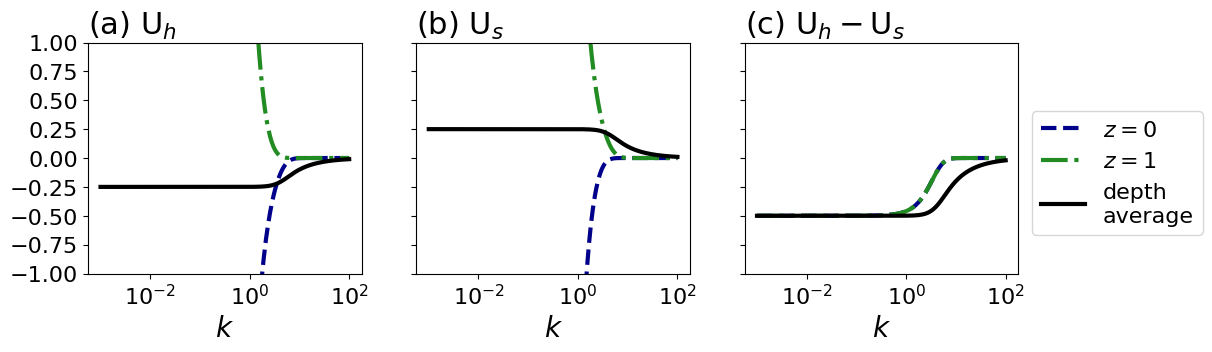
\includegraphics[width=0.99\textwidth]{figs/fig6.png}
\caption{Horizontal velocity response functions $\mathsf{U}_h(k,z)$ and $\mathsf{U}_s(k,z)$,
as well as their difference, at the surface ($z=1$), base ($z=0$), and depth-averaged
over a range of $k$.}
\label{fig:response}
\end{figure}


\section{Some examples}
Finally, we will now look at some steady-state channels and keels. In all of these examples,
we choose a Gaussian-shaped melt rate anomaly that does not vary with time.
Therefore, we set
\begin{align}
m(x,y) = \pm m_0\exp\left(-\frac{1}{2}(x^2+y^2)/\sigma^2\right)
\end{align}
and choose an amplitude of $m_0=3.52\times 10^{-4}$, which corresponds to a melt
rate of 5 m/yr when $H=1000$ m and $\eta = 10^{13}$ Pa s.
In Figures \ref{fig:map}-\ref{fig:keel2}, we look at the effect of
varying the advection parameter $\alpha$, the width of the anomaly via $\sigma$,
and the sign of the anomaly (i.e. melting or freezing). Below, we use the notation $\|\cdot\|_\infty$
to denote the maximum absolute value of a scalar field (i.e. $h$, $s$, $m$) or
maximum flow speed. There is not much else to say right now, so I will
leave the rest to the figures.

\begin{figure}
  \centering
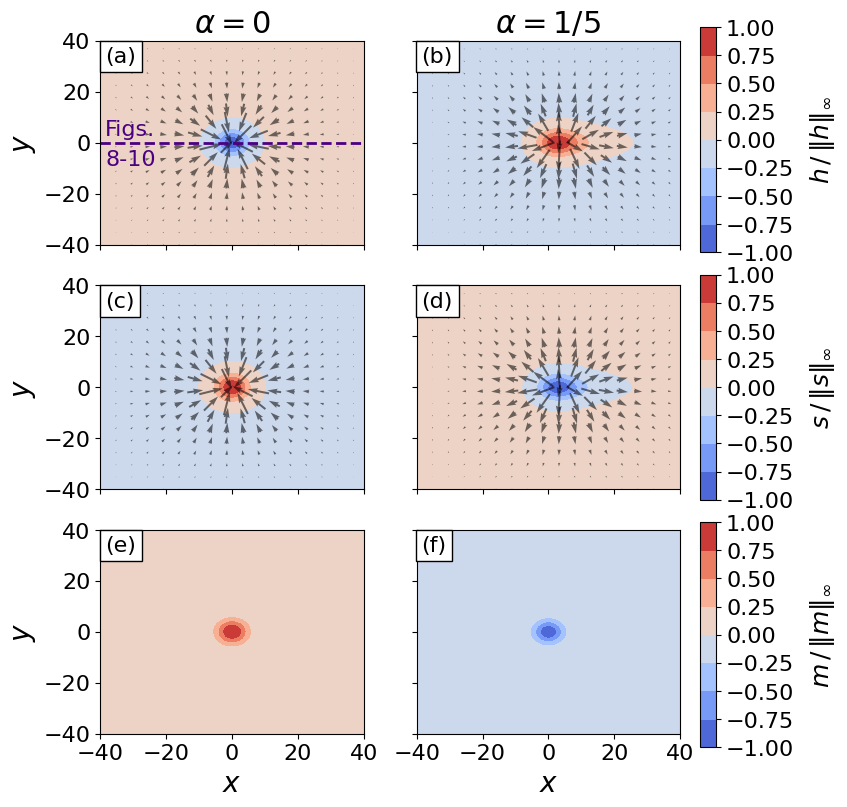
\includegraphics[width=0.99\textwidth]{figs/fig7.png}
\caption{Map-plane plots of steady $h$ and $s$ for two different parameter sets.
Left panels: melting with no background advection. Right panels: freezing with
background advection. Panel (a) shows the $y=0$ centerline where the profiles in Figures \ref{fig:channel}-\ref{fig:keel2} are taken.}
\label{fig:map}
\end{figure}

\begin{figure}
  \centering
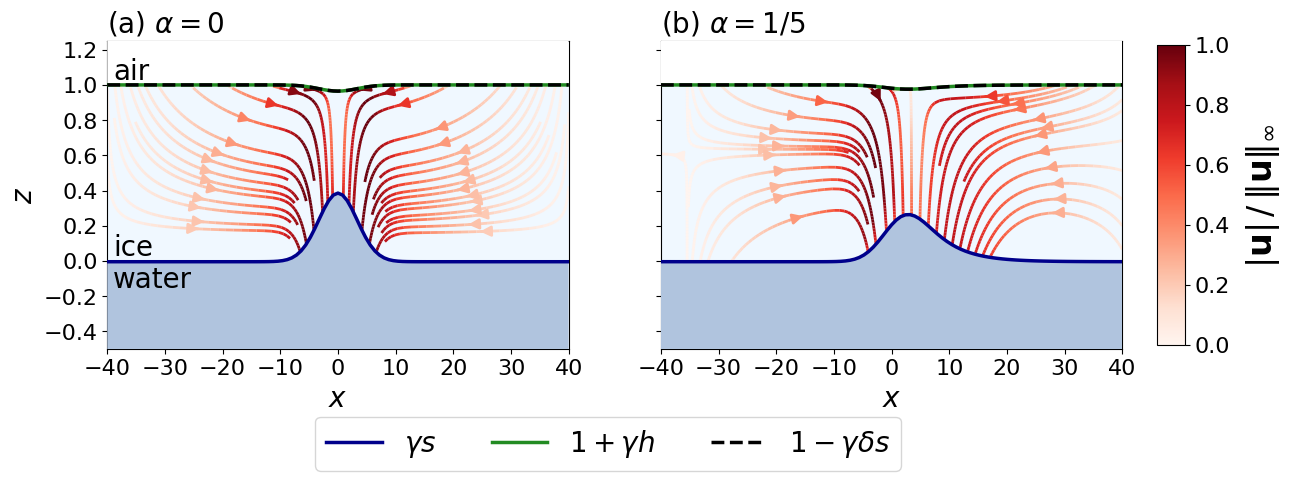
\includegraphics[width=0.99\textwidth]{figs/fig8.png}
\caption{Steady ice-shelf profile highlighting $h$ and $s$, vertically exaggerated by
a factor of $\gamma=50$. The (exaggerated) perfect flotation elevation is shown
as a dashed line. The profiles are taken along the $y=0$ centerline.
Here, $m$ is positive with standard deviation $\sigma = 10/3$.
The in-plane velocity perturbation $[u,w]^T$ streamlines are
plotted on the deformed grid defined by $z\mapsto (1-z)\gamma s + z\gamma h$. }
\label{fig:channel}
\end{figure}

\begin{figure}
  \centering
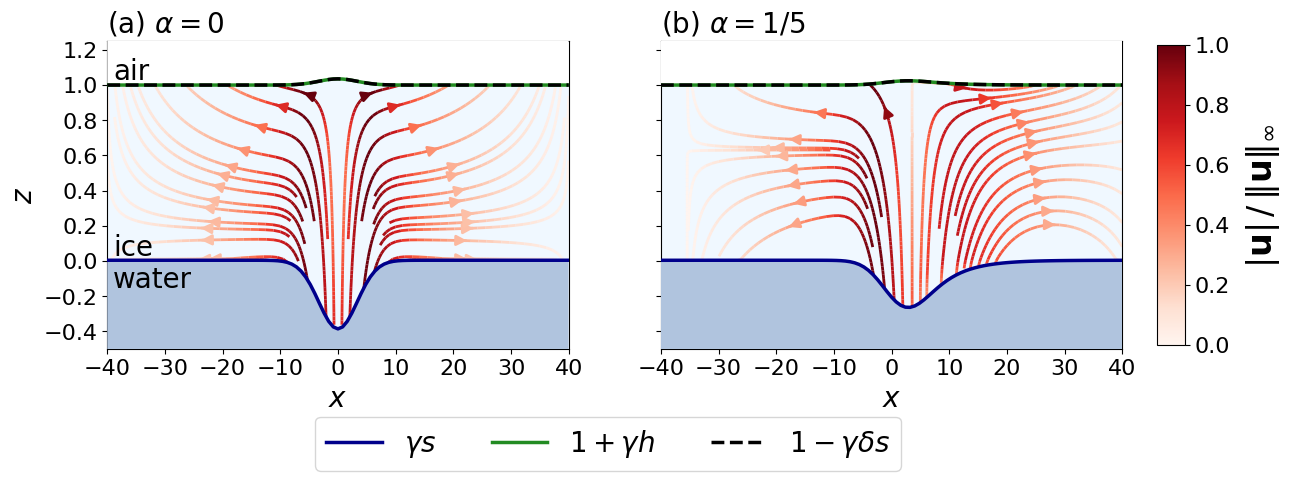
\includegraphics[width=0.99\textwidth]{figs/fig9.png}
\caption{Same as Figure \ref{fig:channel} except with $m<0$. }
\label{fig:keel}
\end{figure}

\begin{figure}
  \centering
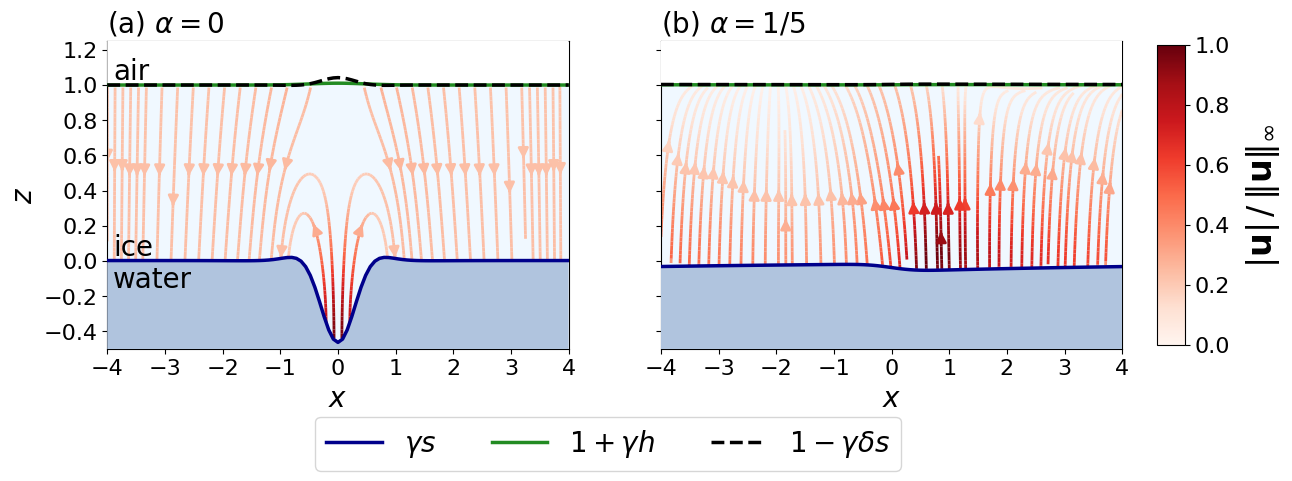
\includegraphics[width=0.99\textwidth]{figs/fig10.png}
\caption{Same as Figure \ref{fig:keel} except with $\sigma = 1/3$
and a smaller vertical exaggeration of $\gamma=30$.}
\label{fig:keel2}
\end{figure}

\clearpage

\section{Appendix: Model derivation}
Here, we derive the model that is introduced in the main text.
We assume that the domain is an ice slab of finite thickness $H$ and infinite horizontal extent.
In $(x,y,z)$-space we assume this ice slab is defined by $|x|<\infty$, $|y|<\infty$, and $s\leq z\leq h$, where $h$ and $s$
are the upper and basal surfaces of the ice sheet, respectively.
We assume that $h$ and $s$ are uniform in the background state.

Assuming Newtonian and incompressible Stokes flow, ice deforms according to
\begin{eqnarray}
&&-p_x + \eta ( u_{xx} +u_{yy} + u_{zz}) = 0 \label{stokesbg1} \\
&&-p_y + \eta ( v_{xx}+v_{yy} + v_{zz}) = 0 \\
&&-p_z + \eta ( w_{xx} +w_{yy} + w_{zz}) = \rho_i g \\
&&u_x + v_y + w_z = 0, \label{stokesbg4}
\end{eqnarray}
where $[u,v,w]^T$ is the velocity, $p$ is the pressure, $\rho_i$ is ice density,
and $g$ is gravitational acceleration.
We assume a stress-free condition at the upper surface ($z=h$), which is equivalent to
\begin{eqnarray}
&&2\eta w_z - p = 0 \label{nostress1}\\
&&\eta(u_z +w_x) = 0 \\
&&\eta(v_z +w_y) = 0.\label{nostress3}
\end{eqnarray}

We consider zero shear stress at the ice-water interface
\begin{eqnarray}
&&u_z + w_x = 0 \label{sl1} \\
&&v_z + w_y = 0 \label{sl2}
\end{eqnarray}
along with a hydrostatic normal stress condition
\begin{eqnarray}
&&p-2\eta w_z  = \rho_w g(\ell-s) \label{hydstress}
\end{eqnarray}
where $\ell$ is sea level.
The upper and basal surfaces of the ice sheet evolve according to kinematic
equations that are coupled to the Stokes flow equations.
The upper surface evolves according to
\begin{eqnarray}
h_t + uh_x + vh_y = w+a,
\end{eqnarray}
where $a$ denotes accumulation or ablation at the ice-sheet surface.
Similarly, the basal surface evolves according to
\begin{eqnarray}
s_t + us_x + vs_y  = w + m \label{stbg}
\end{eqnarray}
where $m$ is the melt rate.

\subsection{Background states}
Perturbations will be taken with respect to a background state (denoted by bars)
corresponding to uniform flow in the $x$ direction and perfect flotation:
\begin{eqnarray}
  &&\bar{u} = \text{constant},\quad \bar{v}=0, \quad \bar{w}=0 \nonumber \\
  &&\bar{h}=H, \quad
  \bar{s}=0,\quad \bar{\ell}  = (\rho_i/\rho_w)H,\quad
  \bar{a} = 0, \quad
\bar{m} = 0.\quad
\end{eqnarray}

\subsection{Perturbation equations}
We introduce perturbations (denoted by 1's) to the background states via
\begin{eqnarray}
&&u= \bar{u} +  u^1, \quad v= \bar{v} +  v^1,\quad w =  \bar{w} + w^1 \nonumber \\
&&p = \bar{p} +  p^1,\quad s =  \bar{s} + s^1, \quad h = \bar{h} +  h^1, \quad m = \bar{m} + m^1, \label{perturbations}
\end{eqnarray}
where the perturbations are assumed to be small.
Note that we aren't considering perturbations to the accumulation/ablation rate.
We obtain equations for the perturbed fields by inserting the perturbations (\ref{perturbations}) into (\ref{stokesbg1})-(\ref{stbg})
and discarding the product terms (i.e., $f^1g^1$).

In this way, we obtain a homogeneous Stokes system for the perturbed fields
\begin{eqnarray}
&&-p_x^1 + \eta (u_{xx}^1 +u_{yy}^1+ u_{zz}^1) = 0 \label{per1} \\
&&-p_y^1 + \eta (v_{xx}^1 +v_{yy}^1+ v_{zz}^1) = 0 \\
&&-p_z^1 + \eta (w_{xx}^1 +w_{yy}^1+ w_{zz}^1) = 0\\
&&u_x^1 + v_y^1 + w_z^1 = 0, \label{per4}
\end{eqnarray}
and the surface kinematic equations become
\begin{eqnarray}
&&h_t^1 + \bar{u} h_x^1  = w^1  \label{ht} \\
&&s_t^1  + \bar{u} s_x^1 = w^1 + m^1. \label{st}
\end{eqnarray}

To account for changes in ice geometry,
we linearize the upper and lower surface boundary conditions at $z=H +  h^1$
and $z= s^1$ onto $z=H$ and $z=0$, respectively.
To do this, we
use a $1^\mathrm{st}$-order Taylor expansion in depth for a function $f(z)$:
$ f(z^0 + z^1) \approx f(z^0) + f_z(z^0)z^1. $
The stress-free condition at $z=H+h^1$ is approximated at $z=H$ by
\begin{eqnarray}
&&2\eta w_z^1 - p^1 = -\rho_i g h^1 \label{pnorm} \\
&&u_z^1 +w_x^1 = 0\label{pshear1}\\
&&v_z^1 +w_y^1 = 0 \label{pshear2}
\end{eqnarray}
Equation (\ref{pnorm}) states that the perturbed normal stress is balanced
by the perturbed cryostatic stress from the elevation anomaly.
Similarly, boundary conditions at the base become
\begin{eqnarray}
&&u_z^1 + w_x^1 = 0  \label{pslaw1}   \\
&&v_z^1 +w_y^1 = 0 \label{pslaw2}\\
&&2\eta w_z^1 - p^1 = \Delta\rho g s^1
\end{eqnarray}
where $\Delta\rho = \rho_w-\rho_i$.
We drop the ``1" superscripts below.

\subsection{Fourier transform approach}
We use the Fourier transform to solve the system (\ref{per1})-(\ref{per4}).
The Stokes flow equation become
\begin{eqnarray}
&&-ik_x\widehat{p} + \eta ( -k^2\widehat{u} + \widehat{u}_{zz}) = 0 \label{pft1} \\
&&-ik_y\widehat{p} + \eta ( -k^2\widehat{v} + \widehat{v}_{zz}) = 0 \\
&&-\widehat{p}_z + \eta (-k^2\widehat{w} + \widehat{w}_{zz}) = 0 \\
&&ik_x\widehat{u} + ik_y\widehat{v} + \widehat{w}_z = 0 \label{pft4}
\end{eqnarray}
Equation (\ref{pft1})-(\ref{pft4}) can be reduced to a fourth-order equation for the transformed vertical velocity
\begin{eqnarray}
&&\widehat{w}_{zzzz} - 2k^2 \widehat{w}_{zz} + k^4 \widehat{w}=0. \label{ode}
\end{eqnarray}
The general solution to (\ref{ode}) is
\begin{eqnarray}
\widehat{w} = \frac{A}{k}e^{k z} + \frac{B}{k}e^{-k z} + {C}ze^{k z}+ {D}ze^{-k z},\label{wformula}
\end{eqnarray}
where the constants $A,B,C,$ and $D$ depend on $k$.
To determine these coefficients, we will rewrite all of the boundary
conditions in terms of $\widehat{w}$ and its $z$ derivatives.
The $z$-derivatives of $\widehat{w}$ are
\begin{eqnarray}
&&\widehat{w}_{z} = {A}e^{k z} - {B}e^{-k z} + {C}e^{k z} + {C}kze^{k z} - {D}kze^{-k z} + {D}e^{-k z} \nonumber \\
&&\widehat{w}_{zz} = {Ak}e^{k z} + {Bk}e^{-k z} + {2Ck}e^{k z} + {C}k^2 ze^{k z} + {D}k^2ze^{-k z} - {2Dk}e^{-k z} \nonumber\\
&&\widehat{w}_{zzz} = {Ak^2}e^{k z} - {Bk^2}e^{-k z} + {3Ck^2}e^{k z} + {C}k^3 ze^{k z} - {D}k^3ze^{-k z} + {3Dk^2}e^{-k z}\nonumber \\ \label{wzzz}
\end{eqnarray}
For later reference,
the surface kinematic equations (\ref{ht})-(\ref{st}) transform to
\begin{eqnarray}
&&\widehat{h}_t + ik_x \bar{u}  \widehat{h} = \widehat{w},\label{hthat}\\
&&\widehat{s}_t +  ik_x \bar{u} \widehat{s} = \widehat{w}+\widehat{m}.\label{sthat}
\end{eqnarray}

The basal shear stress conditions (\ref{pslaw1})-(\ref{pslaw2}) become
\begin{eqnarray}
&&\widehat{u}_z + ik_x \widehat{w} = 0 \label{fslaw1} \\
&&\widehat{v}_z + ik_y \widehat{w} = 0. \label{fslaw2}
\end{eqnarray}
Multiplying (\ref{fslaw1})-(\ref{fslaw2}) by $-ik_x$ and $-ik_y$, respectively, summing the equations, and using the transformed incompressibility condition (\ref{pft4}), we obtain
\begin{eqnarray}
\widehat{w}_{zz} + k^2 \widehat{w} = 0.\label{ftslaw}
\end{eqnarray}
Similarly, the shear stress condition (\ref{pshear1})-(\ref{pshear2}) at the upper surface becomes
\begin{eqnarray}
\widehat{w}_{zz} + k^2 \widehat{w} = 0. \label{ftsstress}
\end{eqnarray}
The normal-stress condition at the upper surface (\ref{pnorm}) transforms to
$
2\eta \widehat{w}_{z} - \widehat{p} = -\rho_i g\widehat{h}.
$
The transformed Stokes equations (\ref{pft1})-(\ref{pft4}) imply that
$-k^2 \widehat{p} = \eta(k^2\widehat{w}_z - \widehat{w}_{zzz}) $, which reduces this expression for
the normal-stress condition to
\begin{eqnarray}
\eta (3k^2 \widehat{w}_{z}-\widehat{w}_{zzz})  = -k^2 \rho_i g \widehat{h}.\label{ftnstress}
\end{eqnarray}
Similar, the normal stress condition at the base becomes
\begin{eqnarray}
\eta (3k^2 \widehat{w}_{z}-\widehat{w}_{zzz})  = k^2 \Delta\rho g \widehat{s}. \label{b4alt}
\end{eqnarray}

To simplify notation, we define the scaled wavevector length $${k'} \equiv kH.$$
Using the formulas (\ref{wformula})-(\ref{wzzz}) evaluated at $z=H$,
the normal stress condition (\ref{ftnstress}) reduces to
\begin{eqnarray}
{A} e^{{k'}} - {B} e^{-{k'}} + {C}{k'} e^{{k'}} - {D}{k'} e^{-{k'}}
=- \frac{\rho_i g }{2\eta }\widehat{h} \equiv b_1, \label{b1}
\end{eqnarray}
and the upper-surface shear-stress condition (\ref{ftsstress}) becomes
\begin{eqnarray}
&&A e^{{k'}} + B e^{-{k'}} + C({k'}+1) e^{{k'}} +D({k'}-1) e^{-{k'}} =  0.
\end{eqnarray}
Using the formulas (\ref{wformula})-(\ref{wzzz}) evaluated at $z=0$,
the lower surface shear stress condition (\ref{ftslaw}) reduces to
\begin{eqnarray}
{A} + {B} + {C}  - {D} = 0.
\end{eqnarray}
Finally the normal stress condition at the base reduces to
\begin{eqnarray}
A-B = \frac{\Delta \rho g}{2\eta}\widehat{s}\equiv b_2. \label{b2}
\end{eqnarray}
The conditions (\ref{b1})-(\ref{b2}) form a linear system for the coefficients $\{A,B,C,D\}$.

Solving for $\{A,B,C,D\}$ symbolically, the vertical velocity at the upper surface is then given by
\begin{eqnarray}
w|_{z=H} =  -\mathsf{R}_f\widehat{h} - \mathsf{B}\delta\widehat{s} \label{wfloat}
\end{eqnarray}
where the surface relaxation function is given by
\begin{eqnarray}
\mathsf{R} = \left(\frac{\rho_i g}{2\eta k}\right) \frac{e^{4{k'}} +4{k'} e^{2{k'}} -1 }{e^{4{k'}} -2(1+2{k'}^2)e^{2{k'}} +1},
\end{eqnarray}
the buoyancy transfer function is given by
\begin{eqnarray}
&&\mathsf{B} = \left(\frac{\rho_i g}{2\eta k}\right) \frac{ 2({k'}+1)e^{3{k'}}+2({k'}-1)e^{{k'}} }{e^{4{k'}} -2(1+2{k'}^2)e^{2{k'}} +1},
\end{eqnarray}
and we have defined
\begin{eqnarray}
&&\delta = \rho_w/\rho_i -1.
\end{eqnarray}
Combining (\ref{hthat}) and (\ref{wfloat}), the upper surface evolves according to
\begin{eqnarray}
\frac{\partial \widehat{h}}{\partial t}+ \left[ik_x \bar{u}  + \mathsf{R}\right]\widehat{h} = -\mathsf{B}\delta\widehat{s}.
\end{eqnarray}
We also have to determine the evolution of the lower surface.
Using $\widehat{w}|_{z=0}= \frac{1}{k}(A+B)$, we obtain
\begin{eqnarray}
\widehat{w}|_{z=0} = -\mathsf{R}\delta\widehat{s} - \mathsf{B} \widehat{h}, \label{wbfloat}
\end{eqnarray}
which, along with (\ref{sthat}), implies that the basal surface evolves according to
\begin{eqnarray}
\frac{\partial \widehat{s}}{\partial t}+ [ik_x\bar{u} + \delta\mathsf{R}]\widehat{s} = \widehat{m} - \mathsf{B} \widehat{h}.
\end{eqnarray}
%
\subsection{Horizontal velocity solutions}
Here we derive the horizontal velocity solutions.
Rearranging the transformed Stokes equations:
\begin{eqnarray}
  &&  \widehat{u}_{zz}-k^2\widehat{u} = \frac{ik_x}{\eta}\widehat{p} \\
  &&  \widehat{v}_{zz}-k^2\widehat{v} = \frac{ik_y}{\eta}\widehat{p}
\end{eqnarray}
These have the general solutions
\begin{eqnarray}
\widehat{u}(z) = \frac{ik_x }{2\eta k} \left(e^{kz}\int_0^z \widehat{p}(z')e^{-kz'}\;\mathrm{d}z' -
e^{-kz}\int_0^z \widehat{p}(z')e^{kz'}\;\mathrm{d}z'\right)
+ E e^{kz} + F e^{-kz} \\
\widehat{v}(z) = \frac{ik_y }{2\eta k} \left(e^{kz}\int_0^z \widehat{p}(z')e^{-kz'}\;\mathrm{d}z' -
e^{-kz}\int_0^z \widehat{p}(z')e^{kz'}\;\mathrm{d}z'\right)
+ G e^{kz} + I e^{-kz}
\end{eqnarray}
where $\{E,F,G,I\}$ depend on the boundary conditions.
As noted before, the body equations (\ref{pft1})-(\ref{pft4}) imply that
\begin{eqnarray}
\widehat{p} = \eta\left(\frac{1}{k^2}\widehat{w}_{zzz}-\widehat{w}_z \right). \label{pexpr}
\end{eqnarray}
We substitute (\ref{pexpr}) into the integrals above
and integrate the $\widehat{w}_{zzz}$ term by parts twice.
To this end, we use the identity
\begin{eqnarray}
\int_0^z \left( \frac{1}{k^2} \widehat{w}_{zzz} - \widehat{w}_{z}\right) e^{\pm kz'}\;\mathrm{d}z'
= \frac{1}{k^2} \left[e^{\pm kz'}\widehat{w}_{zz}\right]_0^z - \frac{\pm k}{k^2}\left[\widehat{w}_ze^{\pm kz'} \right]_0^z
\end{eqnarray}
and find that the pressure integrals reduce to
\begin{eqnarray}
&&e^{kz}\int_0^z \widehat{p}(z')e^{-kz'}\;\mathrm{d}z' -
  e^{-kz}\int_0^z \widehat{p}(z')e^{kz'}\;\mathrm{d}z' \nonumber
  \\ &&= \frac{2\eta}{k} \left( \widehat{w}_z-\widehat{w}_z|_{z=0}\cosh(kz) - \frac{1}{k} \widehat{w}_{zz}|_{z=0}\sinh(kz)  \right).
\end{eqnarray}
Therefore, we obtain
\begin{eqnarray}
&&\widehat{u}(z) = \frac{ik_x }{k^2} P(z)
+ E e^{kz} + F e^{-kz} \label{uexpr}\\
&&\widehat{v}(z) = \frac{ik_y }{k^2} P(z) + G e^{kz} + I e^{-kz} \label{vexpr} \\
&&P(z) = \widehat{w}_z-\widehat{w}_z|_{z=0}\cosh(kz) - \frac{1}{k} \widehat{w}_{zz}|_{z=0}\sinh(kz)
\end{eqnarray}
We can determine the constants $\{E,F,G,I\}$ from the stress boundary conditions.
First, we note that
\begin{eqnarray}
&&\widehat{u}_z(z) = \frac{ik_x }{k^2} P_z(z)
+ E k e^{kz} - F k e^{-kz} \\
&&\widehat{v}_z(z) = \frac{ik_y }{k^2} P_z(z) + G k  e^{kz} - I k e^{-kz} \\
&&P_z(z) = \widehat{w}_{zz}-\widehat{w}_z|_{z=0}k\sinh(kz) - \widehat{w}_{zz}|_{z=0}\cosh(kz)\\
&&P_z(0) = 0 = P(0).
\end{eqnarray}
The stress-free conditions at $z=H$ (i.e., $\widehat{u}_z = -ik_x \widehat{w}$ and
$\widehat{v}_z = -ik_y \widehat{w}$) imply
\begin{eqnarray}
 &&E  e^{{k'}} - F  e^{-{k'}} = -\frac{ik_x}{k^2} \left(k\widehat{w}|_{z=H}+\frac{1}{k}P_{z}(H) \right)\equiv b_3 \label{b4eq}\\
  && G  e^{{k'}} - I  e^{-{k'}} = -\frac{ik_y}{k^2} \left(k\widehat{w}|_{z=H}+\frac{1}{k}P_{z}(H)\right) \equiv b_3'. \label{b4peq}
\end{eqnarray}
For later convenience in deriving the response functions,
we note that $b_3'$ is analogous to $b_3$.
Similarly, the shear stress conditions at the lower surface imply
\begin{eqnarray}
&&E - F  = -\frac{ik_x}{k^2}\left(k\widehat{w}|_{z=0} \right)  \equiv b_5,\\ \label{b5eq}
&&G  -I = -\frac{ik_y}{k^2}(k\widehat{w}|_{z=0}) \equiv b_5'. \label{b5peq}
\end{eqnarray}
As before, we note that $b_4'$ is analogous to $b_4$.
At this point, we can solve symbolically for $\{E,F,G,I\}$.
Then, we can solve for the velocity solutions via (\ref{uexpr})-(\ref{vexpr}).


Using SymPy, the velocities can be written in terms of $\{\widehat{h},\widehat{s}\}$ as
\begin{eqnarray}
\widehat{u} =  \frac{\rho_i g}{2\eta }\frac{ik_x}{k^2}\left(\mathsf{U}_h\widehat{h} +  \mathsf{U}_s\delta\widehat{s}\right) \label{uHf}\\
\widehat{v} = \frac{\rho_i g}{2\eta}\frac{ik_y}{k^2}\left(\mathsf{U}_h\widehat{h} +  \mathsf{U}_s\delta\widehat{s}\right)\label{vHf}
\end{eqnarray}
where the response functions are given by
\begin{align}
&\mathsf{U}_h =  \left[ z(2k'(e^{2k'} + e^{2k'z'}) -(1-z')(e^{2k'(z'+1)} + e^{2k'} - e^{2k'z'} -1 )  )      \right]\mathsf{Q}^{-1}e^{k'}\\
&\mathsf{U}_s =  \left[ z(e^{4k'} +e^{2k'(z'+1)}-e^{2k'}-e^{2k'z'}  ) -(1-z')2k'e^{2k'}(e^{2k'z'}+1)     \right]\mathsf{Q}^{-1}\\
&\mathsf{Q} = e^{{k'z'}}\left(e^{4{k'}} -2(1+2{k'}^2)e^{2{k'}} +1 \right)/k'
\end{align}
where we have defined the scaled height $$z'=H^{-1}z\in[0,1].$$

With the scaling in the main text, the above equations
take the nondimensional form
\begin{eqnarray}
\widehat{u} =  \frac{ik_x}{k^2}\left(\mathsf{U}_h\widehat{h} +  \mathsf{U}_s\delta\widehat{s}\right), \label{uHf}\\
\widehat{v} = \frac{ik_y}{k^2}\left(\mathsf{U}_h\widehat{h} +  \mathsf{U}_s\delta\widehat{s}\right),\label{vHf}
\end{eqnarray}
noting that the response functions are already nondimensional.

\end{document}
